\chapter{Manager manual}
In this part, installation and basic usage guide will be presented.
\section{Installation}
Download application \emph{DigitalLighterServer} from Android Play store\footnote{\url{TODO}} and install this application on your Android device.
\section{Usage}
After starting the server application, you will see screen similar to Figure \ref{fig:manual_server0}.
\begin{figure}[h]
	\centering
		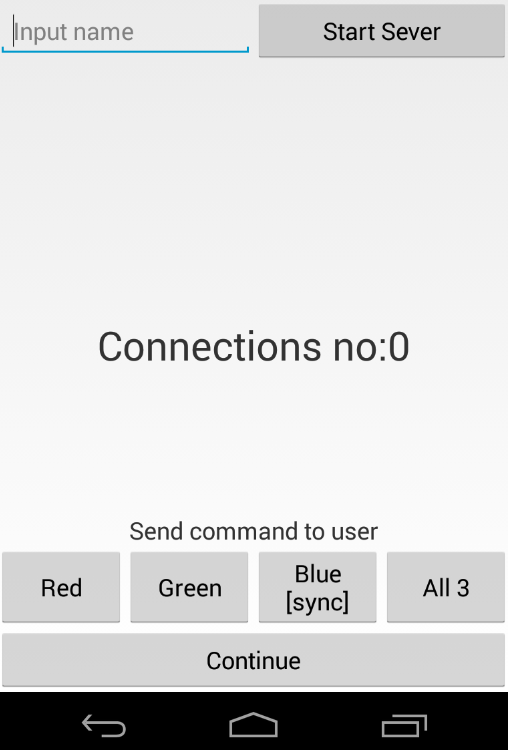
\includegraphics[width=5cm]{appendix/server0.png}
	\caption{Create server screen}
	\label{fig:manual_server0}
\end{figure}

First step you as a manager you want to do is create a new service.
This can be done by typing a name (e. g. concert stage name or artist's name) into the input box and pressing button \emph{Start Server} as shown in Figure \ref{fig:manual_server1}.

\begin{figure}[h]
	\centering
		
\includegraphics[width=5cm]{appendix/server2.png}
	\caption{Choose name of a server}
	\label{fig:manual_server1}
\end{figure}

After this action, client users can connect to this server.
For every connected client, \emph{Connections no} count will increase and therefore you can see how many people want to be involved in your light show.

By pressing buttons \emph{Red}, \emph{Green}, \emph{Blue} and All 3 you can see what is the distribution of connected phones in area. 
After pressing a button, the clients will lit with appropriate color.
You can also see the delay of network by using colors \emph{Red} and \emph{Green}, which are played immediately when client receive  that command.
On the other hand, \emph{Blue} command is synchronized.
Whenever you are ready, you can continue by clicking on button \emph{Continue}.
This will lead you to new screen, which can be seen in Figure \ref{fig:manual_server2}.

\begin{figure}[h]
	\centering
		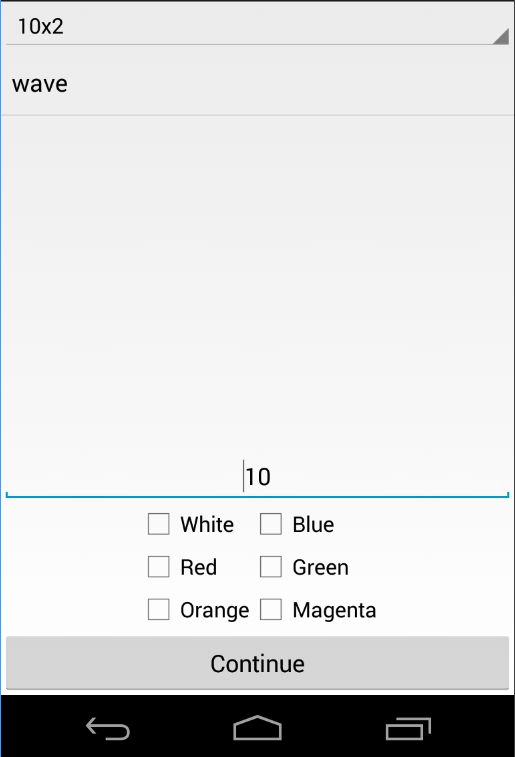
\includegraphics[width=5cm]{appendix/server4.png}
	\caption{Choosing media screen}
	\label{fig:manual_server2}
\end{figure}

In this screen you can choose media to be played by first choosing appropriate grid size from first list.
After that a second list with concrete media is updated according to grid size and you have to choose specific item.
After that, in next input field you can change FPS\footnote{Frames Per Second} value and last you can choose which colors should be used for detection of position of devices.

When you are ready, you can continue by clicking on button \emph{Continue}.
This will take you into last screen, similar to Figure \ref{fig:manual_server3}.
\begin{figure}[h]
	\centering
		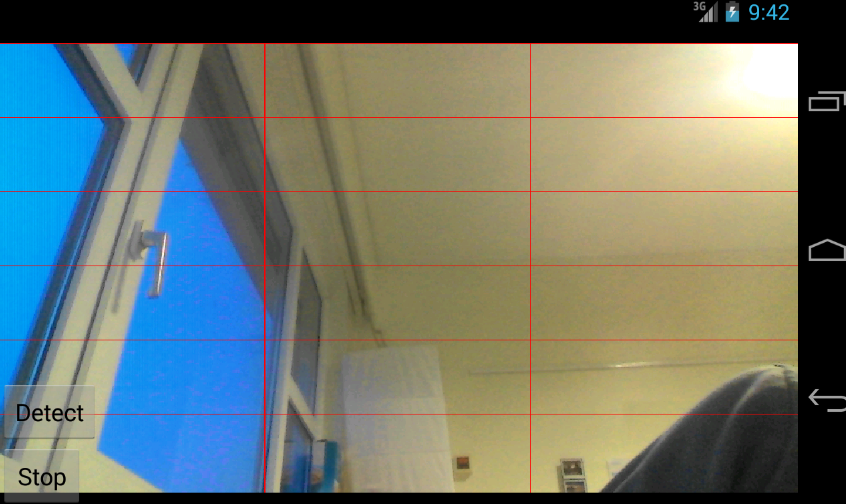
\includegraphics[width=12cm]{appendix/server9.png}
	\caption{Camera screen}
	\label{fig:manual_server3}
\end{figure}

In this screen, there you can see realtime output from camera on your mobile phone.
You can also see the grid and two buttons \emph{Detect} and \emph{Stop}.
When you are ready, just position the camera in a way, that the audience is in screen, and click on button \emph{Detect}.
Now, you have hold still the so the clients' mobile devices do not change particular tile in grid.
Detection of position can take a while, the length is dependent on number of connected clients.
After the detection is ready, the media you have chosen will immediately starts to play on clients.
When you have enough of fun, you can pres \emph{Stop} button, and then use classic Android button for returning to previous screen and choose different parameters of media playing and repeat the process.

\chapter{Client user manual}
In this part, installation and usage guide will be presented.
\section{Installation}
Download application \emph{DigitalLighter} from Android Play store\footnote{\url{TODO}} and install this application on your Android device.
\section{Usage}
After starting the application you can see screen similar to one shown in Figure \ref{fig:manual_client}

\begin{figure}[h]
	\centering
		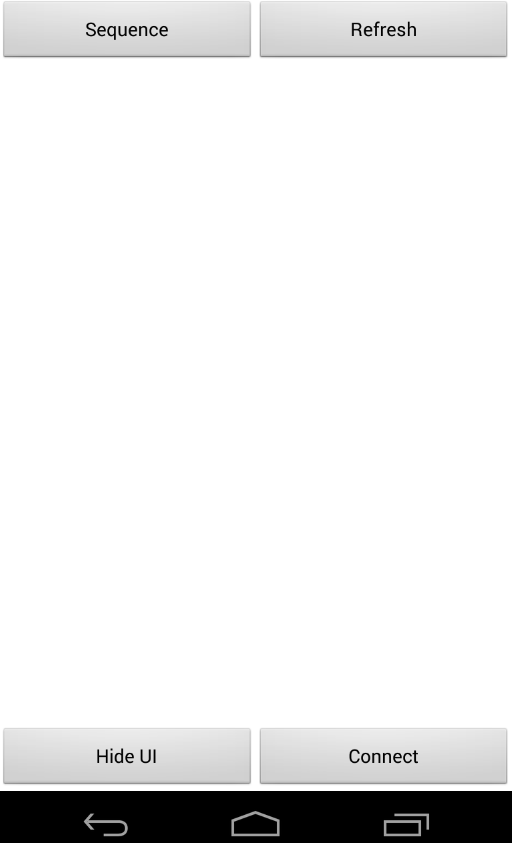
\includegraphics[width=5cm]{appendix/client1.png}
	\caption{Clients screen}
	\label{fig:manual_client}
\end{figure}

When you are ready to connect to service, simply click on button \emph{Refresh}, which will cause refreshing the list of available servers. 
Since that moment, the list is updated automatically.
Choose your server and click on button \emph{Connect}.
From this moment, the colors of your screen are controlled by remote server.
You can improve better impression from light show by clicking on button \emph{High UI}, which will cause hiding of all control buttons and server list.
When you do not want to participate in light show, you can disconnect by clicking on button \emph{Disconnect}.
Note, that this button will appear only, when you are already connected to some server.
